% !TEX root = ./../../../_Thesis.tex

\begin{figure*}[!t]
	\centering

	\begin{tabular}{@{}r@{ } c@{ } c@{ } c@{ } c@{ } c }
	&
	\small{-0.00 D} &
	\small{-1.00 D} &
	\small{-2.00 D} &
	\small{-3.00 D} &
	\small{-4.00 D} & \\

	\begin{sideways} \parbox[b]{20mm} {Camera} \end{sideways} &
	
\includegraphics[width=0.185\textwidth]{__Images/05/BW_N(20-200)_-0D_to_-4D/bw_N_20-200_Camera-0,00D(lens).png} &
	
\includegraphics[width=0.185\textwidth]{__Images/05/BW_N(20-200)_-0D_to_-4D/bw_N_20-200_Camera-1,00D(lens).png} &
	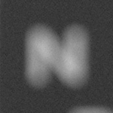
\includegraphics[width=0.185\textwidth]{__Images/05/BW_N(20-200)_-0D_to_-4D/bw_N_20-200_Camera-2,00D(lens).png} &
	
\includegraphics[width=0.185\textwidth]{__Images/05/BW_N(20-200)_-0D_to_-4D/bw_N_20-200_Camera-3,00D(lens).png} &
	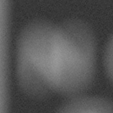
\includegraphics[width=0.185\textwidth]{__Images/05/BW_N(20-200)_-0D_to_-4D/bw_N_20-200_Camera-4,00D(lens).png} \\

	\begin{sideways} \parbox[b]{20mm} {Simulation} \end{sideways} &
	
\includegraphics[width=0.185\textwidth]{__Images/05/BW_N(20-200)_-0D_to_-4D/bw_N_20-200_Camera-0,00D(simulated).png} &
	
\includegraphics[width=0.185\textwidth]{__Images/05/BW_N(20-200)_-0D_to_-4D/bw_N_20-200_Camera-1,00D(simulated).png} &
	
\includegraphics[width=0.185\textwidth]{__Images/05/BW_N(20-200)_-0D_to_-4D/bw_N_20-200_Camera-2,00D(simulated).png} &
	
\includegraphics[width=0.185\textwidth]{__Images/05/BW_N(20-200)_-0D_to_-4D/bw_N_20-200_Camera-3,00D(simulated).png} &
	
\includegraphics[width=0.185\textwidth]{__Images/05/BW_N(20-200)_-0D_to_-4D/bw_N_20-200_Camera-4,00D(simulated).png} \\

	\begin{sideways} \parbox[b]{20mm} {Local~SSIM} \end{sideways} &
	
\includegraphics[width=0.185\textwidth]{__Images/05/BW_N(20-200)_-0D_to_-4D/bw_N_20-200_Camera-0,00D(comparison).png} &
	
\includegraphics[width=0.185\textwidth]{__Images/05/BW_N(20-200)_-0D_to_-4D/bw_N_20-200_Camera-1,00D(comparison).png} &
	
\includegraphics[width=0.185\textwidth]{__Images/05/BW_N(20-200)_-0D_to_-4D/bw_N_20-200_Camera-2,00D(comparison).png} &
	
\includegraphics[width=0.185\textwidth]{__Images/05/BW_N(20-200)_-0D_to_-4D/bw_N_20-200_Camera-3,00D(comparison).png} &
	
\includegraphics[width=0.185\textwidth]{__Images/05/BW_N(20-200)_-0D_to_-4D/bw_N_20-200_Camera-4,00D(comparison).png} \\
	
	\begin{sideways} \parbox[b]{20mm} {Difference} \end{sideways} &
	
\includegraphics[width=0.185\textwidth]{__Images/05/BW_N(20-200)_-0D_to_-4D/bw_N_20-200_Camera-0,00D(diff).png} &
	
\includegraphics[width=0.185\textwidth]{__Images/05/BW_N(20-200)_-0D_to_-4D/bw_N_20-200_Camera-1,00D(diff).png} &
	
\includegraphics[width=0.185\textwidth]{__Images/05/BW_N(20-200)_-0D_to_-4D/bw_N_20-200_Camera-2,00D(diff).png} &
	
\includegraphics[width=0.185\textwidth]{__Images/05/BW_N(20-200)_-0D_to_-4D/bw_N_20-200_Camera-3,00D(diff).png} &
	
\includegraphics[width=0.185\textwidth]{__Images/05/BW_N(20-200)_-0D_to_-4D/bw_N_20-200_Camera-4,00D(diff).png} \\

	\end{tabular}
	
	\caption[Comparisons of our simulated results against ground truth obtained with a hyperopic camera]{Comparisons of our simulated results against ground truth obtained with a hyperopic camera. These images correspond to a Snellen ratio of 20/200. (top row) Images captured using the DSLR camera with extra lenses varying from 0.0 to 4.0 diopters. (second row) Our simulated results. (third row) SSIM metric results. (fourth row) AD metric.}
	\label{fig:comparison_hyperopic_bw}
\end{figure*}
